%Typeset using XeLaTeX

\documentclass[10pt,a4paper]{book}
\usepackage{mathtools,amssymb,amsthm}
%\usepackage{phonetic}
\usepackage{fancyhdr}
\usepackage[pass]{geometry}
\usepackage{fontspec}
%\usepackage{xunicode}
%\usepackage{xltxtra}
%\usepackage{xgreek}
\setmainfont[Mapping=TeX-text]{Times New Roman}
\usepackage{hyperref}
%\usepackage{color}
\usepackage[Glenn]{fncychap}
\ChNameVar{\bfseries\Large}
%\usepackage{tabularx}
%\usepackage[normalem]{ulem}

%\usepackage{tikz}
\usepackage{enumerate}
\usepackage{natbib}

\renewcommand{\maketitle}{
	\begin{titlepage}
		\newgeometry{left=4cm, top=2.3cm, bottom=2.3cm}
		\hbox{\mbox{\hspace{-1.3cm}}
			\vrule depth 0.98\textheight
			\mbox{\hspace{1cm}}
			\vtop{
				\vspace{2cm}
				\begin{flushleft}
					\huge{\bf Pricing Games in Heterogeneous 2-link Parallel Networks\\}
					\vskip3cm
					\Large  Thomas Pappas\\
					AL1.18.0011\\
					\vskip3cm
					\begin{minipage}{7.5cm}
						\begin{flushleft}
							\normalsize {\it {\bf Examination committee:}\\
								Dimitris Fotakis, School of Electrical and Computer Engineering, National Technical University of Athens.\\
								Professor's name, Department or School, Institution.\\
								Professor's name, Department or School, Institution.}
						\end{flushleft}
					\end{minipage}
					\hskip0.5cm
					\begin{minipage}{6cm}
						\begin{flushleft}
							\normalsize {\it {\bf Supervisor:}\\
								Dimitris Fotakis, Professor, \\ School of Electrical and Computer Engineering,\\
								National Technical University of Athens.\\
							}
						\end{flushleft}
					\end{minipage}
				\end{flushleft}
				\vskip6cm
				\hskip4.5cm
				\begin{minipage}{5cm}
					\begin{center}
						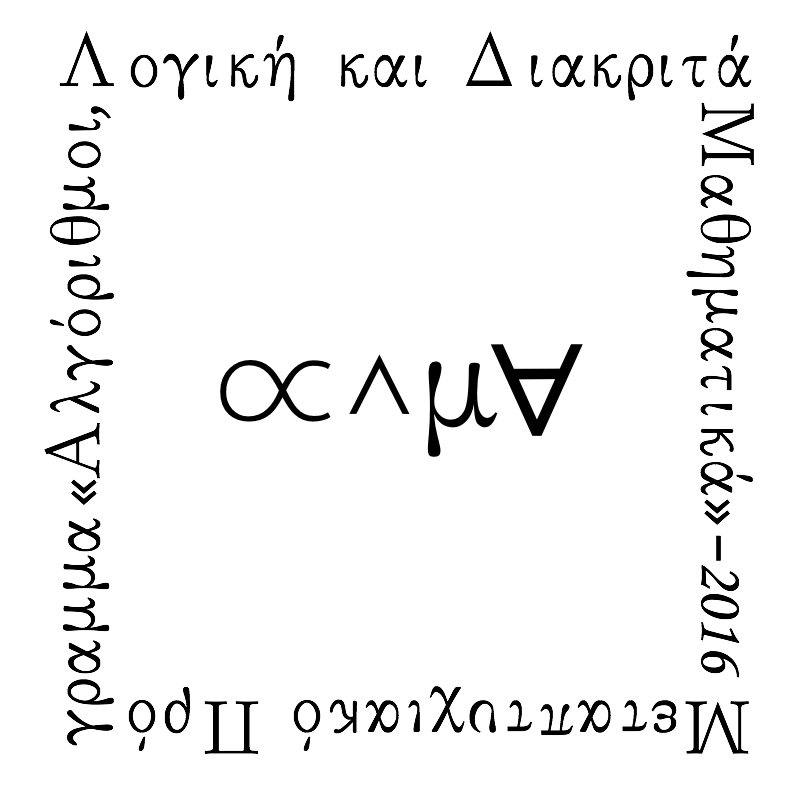
\includegraphics[width=0.8\textwidth]{alma.png}
					\end{center}
		\end{minipage}}}
	\end{titlepage}
}

% Commands for wrapping properly common expressions.
\newcommand{\indeq}[1]{\stackrel{\text{#1}}{=}}
\newcommand{\RightarrowArg}[1]{\stackrel{#1}{\Rightarrow}}
\newcommand{\LeftrightarrowArg}[1]{\stackrel{#1}{\Leftrightarrow}}
\newcommand{\NE}{\mathrm{N.E.}}
\newcommand{\as}{\mathrm{\alpha_s}}
\newcommand{\R}{\mathbb{R}}
\newcommand{\Gm}{\mathcal{G}}
\DeclareMathOperator*{\argmax}{arg\,max}
% \newcommand{\Exp}{\mathrm{Exp}}
% \newcommand{\Expect}{{\rm I\kern-.3em E}}

% Theorem structures.
\theoremstyle{definition}
\newtheorem{ex}{}[section]
\newtheorem{definition}{Definition}[chapter]
\newtheorem{theorem}[definition]{Theorem}
\newtheorem{lemma}[definition]{Lemma}
\newtheorem{corollary}[definition]{Corollary}
\theoremstyle{comment}
\newtheorem{example}[definition]{Example}
\newtheorem{claim}[definition]{Claim}

\fancyhead[LO]{\slshape \leftmark}
\fancyhead[RE]{\slshape \rightmark}
\fancyhead[LE]{}
\fancyhead[RO]{}
\fancyfoot[LO,RE]{\tiny{\it}}

% Main document
\begin{document}

\maketitle
\clearpage


\thispagestyle{empty}
\null
\clearpage

\restoregeometry

\thispagestyle{empty}
\pagenumbering{gobble}
\chapter*{Abstract}
In this masters thesis we study a $2$-level optimisation problem where, on a $2$-link network from a source $s$ to a target $t$, a unit of flow wants to move from $s$ to $t$ using the link with the lowest cost, while the two link owners compete for profit by assigning tolls to links and thus creating a toll congestion game.
We examine only affine latencies for the links.
In addition, each flow player responds to tolls in a heterogeneous way, i.e. each flow player $p$ has a different money-time sensitivity value, which is described by a distribution function $\alpha(p)$.
First we present some basic definitions and properties of profit homogeneous games.
Using them as base, we examine cases of fixed and step distribution functions, where for the latter we present strict conditions for the existence or not of a Nash Equilibrium.
We then introduce a new term, the split function $\as(t)$, defined as the time-money sensitivity value for which the $2$ link costs are equal for a given set of tolls $t$. With the help of $\as$ we will describe and prove some properties of the heterogeneous games for continuous distribution functions.
In our main result, we generalise the conditions necessary for the existence of a Nash Equilibrium in the profit game between the toll owners, and finally we discuss some extensions to $n$-link parallel networks.
\clearpage

\thispagestyle{empty}
\null
\clearpage

\thispagestyle{empty}
\pagenumbering{gobble}
\chapter*{Συνοψη}
Σε αυτή τη διπλωματική μεταπτυχιακού μελετάμε ένα πρόβλημα βελτιστοποίησης $2$ επιπέδων, όπου σε ένα δίκτυο με $2$ ακμές από μια πηγή $s$ σε ένα στόχο $t$, μια μονάδα ροής θέλει να μετακινηθεί από το $s$ στο $t$ χρησιμοποιώντας την ακμή με το χαμηλότερο κόστος, ενώ οι δύο ιδιοκτήτες των ακμών ανταγωνίζονται για κέρδος βάζοντας δίοδια στις ακμές και δημιουργώντας έτσι ένα παίγνιο συμφόρησης με διόδια.
Εξετάζουμε μόνο αφινικές καθυστερήσεις για τις ακμές.
Επιπλέον, ο κάθε παίκτης ροής αντιδρά στα διόδια με ετερογενή τρόπο, δηλ. ο κάθε παίκτης ροής $p$ έχει διαφορετική τιμή ευαισθησίας χρόνου-χρήματος, η οποία περιγράφεται από μια συνάρτηση κατανομής $\alpha(p)$.
Πρώτα παρουσιάζουμε κάποιους βασικούς ορισμούς και ιδιότητες των ομογενών παιγνίων κέρδους. Mε αυτά ως βάση, εξετάζουμε περιπτώσεις σταθερών και βηματικών συναρτήσεων κατανομής, όπου για το τελευταίο παρουσιάζουμε αυστηρές συνθήκες για την ύπαρξη ή μη σημείου ισορροπίας Nash.
Μετά εισαγάγουμε έναν νέο όρο, τη συνάρτηση διαχωρισμού $\as(t)$, ορισμένη ως η τιμή ευαισθησίας χρόνου-χρήματος για την οποία τα κόστη των $2$ ακμών είναι ίσα για ένα δοσμένο σετ διοδίων $t$.
Με τη βοήθεια της $\as$ θα περιγράψουμε και θα αποδείξουμε μερικές ιδιότητες των ετερογενών παιγνίων με συνεχή συνάρτηση κατανομής.
Στο κύριο αποτέλεσμά μας, γενικοποιούμε τις συνθήκες που είναι απαραίτητες για την ύπαρξη ισορροπίας Nash στο παίγνιο κέρδους μεταξύ των ιδιοκτητών των ακμών, και τελικώς συζητάμε κάποιες επεκτάσεις για δίκτυα με $n$ ακμές.
\clearpage

\thispagestyle{empty}
\null
\clearpage

\pagestyle{fancy}

\pagenumbering{roman}
\tableofcontents
\clearpage

\thispagestyle{empty}
\null
\clearpage

\pagenumbering{arabic}


\chapter{Introduction}

In this thesis we study a three level optimisation problem.
On the basis there is a 2-node $(s, t)$, 2-link $s-t$ network, each link with a non-decreasing latency function that defines how the traffic increases as more players flow into that link.
On the first level a flow $[0, 1]$ wants to move from $s$ to $t$ and experience the minimum latency (traffic).
On the second level, the links might also have tolls which impose an additional cost to the flow players, plus in our case (heterogeneous users) each player has a different money-time trade-off and thus see the link costs differently.
Finally on the third level (are the levels really that way?), the tolls are owned by players who profit on the flow that uses that link and compete to maximise it.

We know from Cole et al. \cite{10.1145/780542.780618} that regardless of the distribution function $a$ or the latency functions (as long as they are non-decreasing) a $\NE$ always exists.
In that $\NE$ the users are split with the money-sensitive ones on the link with the lower toll and the time-sensitive ones on the higher toll one, each one seeing their link as either lower or equal cost with the other (while they all see traffic equally).

We introduce a new term $\as=\frac{l_1(x)-l_2(1-x)}{t_2-t_1}$ which is the $a(p)$ value of a user $p$ which sees the link costs equally.


\section{Related Work}

Adding tolls to a Network Game has began as a standard practice to regulate the network flow, as it is well known that the equilibrium that occurs by the game is not guarranteed to be the most efficient.

TODO

\cleardoublepage


\chapter{Preliminaries}

In this section we will describe the model utilised throughout this thesis.
If we attempted to call that model by including all of it's properties, the result would be a Heterogeneous Non-atomic 2-link Parallel Network Toll Congestion Pricing Game, so while we will describe each of those properties, we will eventually focus on heterogeneity and the pricing competition, thus calling it a Heterogeneous Pricing Game.

\section*{Non-atomic Parallel Network Games}

We consider a directed graph $G = (\{s, t\}, N)$ where $N = \{1,\dots, n\}$ is a set of parallel links from a source node $s$ to a target node $t$.
For the non-atomic case, there is one unit of traffic that wishes to travel from $s$ to $t$, described as the unit interval $[0, 1]$ endowed with Lebesque measure $\lambda$.
Each point $p \in [0, 1]$ will be called a \textit{player} and will be considered to be non-cooperative and contribute to the traffic by an infinitesimal amount.
As such the decisions of individual players have no effect on the game and it becomes natural to only consider non-zero measure collection of players.

A \textit{flow} is a Lebesque measurable function $f: [0, 1] \rightarrow N$ that describes which link is selected by each player.
It is more intuitive, however, to consider the resulting flow on each link (\textit{flow on paths}), i.e. $x_i = \lambda(\{p \in [0, 1]: f(p) = i\})$.
Hence we get flow as a (stochastic) vector $x = (x_i)_{i \in N}$ where $x_i$ is the total flow on link $i$ with $x_i \geq 0$ and $\sum_{i \in N}x_i = 1$.
The flow then creates congestion on the links, each described by a non-decreasing latency function $(\ell_i)_{i \in N}$ which we assume to be affine.
We denote by $\mathcal{L}_d$ the class of polynomial latency functions with nonnegative coefficients and degree at most $d$, and as such $\mathcal{L}_1$ becomes the class of affine latency functions.
Finally, the network can also be extended by allowing a set of tolls $t = (t_i)_{i \in N}$ to be assigned to each link, which in turn adds to the effective cost of a player using them.

The above set-up creates a Non-atomic Parallel Network Game with tolls where each player will select the edge that minimises their \textit{individual} traffic latency.
We consider two cases where players either react to tolls in a \textit{homogeneous} or a \textit{heterogeneous} manner.

\subsection*{Homogeneous players}

In the homogeneous case all players have an equal reaction to tolls, and therefore the effective cost of a player using link $i$ becomes $\ell_i(x_i) + t_i$.
For a given set of tolls $t$, a flow $x$ is a \textit{Wardrop equilibrium for $t$} if $\forall i, j \in N$ with $x_i > 0$ it holds that
\begin{equation}
	\label{wardrop_inequality_cost}
	\ell_i(x_i) + t_i \leq \ell_j(x_j) + t_j
\end{equation}
In that case, all links with $x_i > 0$ have equal effective costs, i.e. there exists some $K > 0$ such that $\ell_i(x_1) + t_i = K$ for all links $i$ with $x_i > 0$.
From a well-known result from Beckman et al. \cite{beckmann1956studies} and Dafermos and Sparrow \cite{1363388843888284416}, such and an equilibrium for $t$ exists and is unique, therefore for a toll vector $t$ we can denote by $x(t)$ the flow occurring on  that unique equilibrium for the given toll $t$.
We will freely use when needed the general game-theoretical notation of $x(t_i, t_{-i})$ where $t_{-i} = t \setminus \{t_i\}$.
We copy Lemma 2.1 from Harkes et al \cite{Harks_2019} as is for later use.
\begin{lemma}
	\label{lemma:wardrop_equilibrium}
	A flow $x$ is a Wardrop equilibrium for $t$ if and only if for all feasible flows $x^\prime$,
	\[\sum_{i \in N} (\ell_i(x_i) + t_i) \cdot (x_i - x_i^\prime) \leq 0\]
\end{lemma}
If $t = 0$ then the equilibrium is called the \textit{Wardrop equilibrium}.
It's also worth noting that looking at \eqref{wardrop_inequality_cost}, we can see that what actually matters, with regard to the flow, is the relative difference among the tolls.
I.e. if we consider any $c \in \R_+$ (or even $c \geq -\min_{i \in N} t_i$) then for $t^\prime = t + c$ the inequalities remain true for all $i, j \in N$ and thus the network game for the flow between tolls $t$ and $t^\prime$ is the same.

Finally for affine latencies we can calculate $x(t)$.
For $l_i(x_i) = a_i \cdot x_i + b_i, a_i > 0, b_i \geq 0$ and $t \in \R_+^N$ define $N(t) = \{i \in N | x_i(t) > 0\}$.
Since $x(t)$ is an equilibrium for $t$ and $\sum_{i \in N(t)}x_i(t) = 1$ we solve the equations with regard to the common efficient cost $K$ and then we get for all $i \in N(t)$
\begin{equation}
	x_i(t) = \frac{1 + \sum_{j \in N(t)}\frac{b_j + t_j - b_i - t_i}{a_j}}{\sum_{j \in N(t)}\frac{a_i}{a_j}}
\end{equation}

\subsection*{Heterogeneous players}

In the heterogeneous case, each player $p$ reacts differently to tolls, presumably due to different money/time valuation ratios.
We describe this by adding a money-sensitivity weight $\alpha(p)$ on the toll costs experienced by the player, making them see the cost of each edge as $c_i^p(t) = \ell_i(x_i(t)) + \alpha(p) \cdot t_i$ and then seek the shortest link among them.
By also assuming that the players are sorted by money-sensitivity, we can describe their heterogeneity by defining a non-decreasing function $\alpha: [0, 1] \rightarrow [0, \infty]$.
We call $\alpha$ a \textit{distribution function}.
Even though the definition does allow functions that are not upper bounded with $\alpha(1) = +\infty$, we will always assume that $\alpha$ is finite on $[0, 1)$.
Finally, we will assume that $\alpha(0) > 0$, since, as we'll see in more detail in Lemma \ref{lemma:a_0_0}, allowing many players close to $0$ breaks the pricing game.

We can therefore define an instance of a Heterogeneous Pricing Game as the tuple $(N, \ell, \alpha)$ with $N = \{1, 2, \dots, n\}$, $\ell = (\ell_i)_{i \in N}$ and $\alpha$ the distribution function.
Then with all the above we can again define a Nash equilibrium for the game if $\forall i \in N$ and $\forall p \in [0, 1]$ it holds that
\[c_{f(p)}^p(t) \leq c_i^p(t)\]
Existence of an equilibrium is guaranteed by the more general results of Schmeidler \cite[Thm 2]{1973JSP.....7..295S}, while uniqueness is covered by Milchtaich \cite[Prop 3.3]{doi:10.1287/moor.25.3.349.12220}; for a more detailed coverage of those look at the definitions and propositions of Cole et al. \cite[\S2]{10.1145/780542.780618}.
Therefore can extend the definition for $x(t)$ similarly as in the homogeneous case.

Finally, we will prove here a general property of parallel networks which capture the relationship between latencies and tolls.
It is trivial for homogeneous games that higher tolls create lower latencies on the respective edges, but for the heterogeneous case it is not straightforward so we'll prove it.

\begin{lemma}
	\label{lemma:latencies_tolls}
	For a Heterogeneous Parallel Game $(N, \ell, \alpha)$ with tolls $t$ and Nash equilibrium for $t$ flow $x(t)$, it holds that for all $i, j \in N$ with $x_i(t), x_j(t) > 0$
	\begin{enumerate}[(i)]
		\item $\ell_i(x_i(t)) < \ell_j(x_j(t))$ iff $t_i > t_j$
		\item $\ell_i(x_i(t)) = \ell_j(x_j(t))$ iff $t_i = t_j$
		\item $\ell_i(x_i(t)) > \ell_j(x_j(t))$ iff $t_i < t_j$
	\end{enumerate}
\end{lemma}

\begin{proof}
	We will prove $(i)$ and the rest follow similarly.
	For the left-to-right direction we assume that $\ell_i(x_i(t)) < \ell_j(x_j(t))$.
	If now $t_i \le t_j$ then for all players $p$ we get $\ell_i(x_i(t)) + \alpha(p) \cdot t_i < \ell_j(x_j(t)) + \alpha(p) \cdot t_j \Rightarrow c_i^p(t) < c_j^p(t)$.
	Therefore there exist players $p_j$ on link $j$ for which $c_{f(p_j)}^{p_j}(t) = c_j^{p_j}(t) > c_i^{p_j}(t)$, which is a contradiction since $x(t)$ is a Nash equilibrium.
	The opposite direction is also proved similarly.
\end{proof}

\section*{Pricing Games}

While keeping the above Network Game model, we introduce $n$ agents who each own one link of the network and can thus assign its toll and profit from it.
The profit is defined for each link owner $i$ as $\Pi_i = x_i \cdot t_i$ which, since we defined $x(t)$ above, we can extend the definition to $\Pi_i(t) = x_i(t) \cdot t_i$ describing the profit at the equilibrium for given toll $t$.
The link owners compete with each other for profit, each selfishly selecting the toll $t_i$ that will maximise their profit given the remaining tolls $t_{-i}$.
We describe this best response as $B_i(t_{-i}) = \argmax_{t_i \geq 0} \Pi_i(t_i, t_{-i})$.
Consequently, a toll vector $t$ is a \textit{Nash Equilibrium} for the pricing game, if $\forall i \in N$ and $\forall t_i^\prime \in \R$ it holds that
\[\Pi_i(t_i, t_{-i}) \geq \Pi_i(t_i^\prime, t_{-i})\]

\subsection*{Homogeneous players}

For homogeneous players and affine latencies we can calculate the best response functions for each link owner by solving first order conditions on $\Pi_i(t_i, t_{-i})$ for $t_i$. TODO

\section*{2-link Heterogeneous Pricing Games (our model)}

Focusing on the model that will be used in this thesis, we simplify our network by only having $2$ links, and then consider that the flow is acting in a heterogeneous way.
The model can thus be defined as the tuple $([2], \ell, \alpha)$, where $[2] = \{1, 2\}$ the links, $\ell = (\ell_1, \ell_2)$ the latency functions and $\alpha$ the distribution function.
[TODO: Add figure]
When discussing properties of the model where the pricing game is not relevant, we will refer to a $([2], \ell, \alpha)$ instance as a toll game, and otherwise as a pricing game.


\chapter{Money sensitivity split}

\section{Introduction}

Consider a $([2], \ell, \alpha)$ toll game such that $x_1(0), x_2(0) > 0$ with tolls $t = (t_1, t_2)$ assigned to them and  $x(t) = (x_1(t), x_2(t))$ the Nash equilibrium for $t$.
Without loss of generality we assume $t_1 > t_2$ which from Lemma \ref{lemma:latencies_tolls} follows that $\ell_1(x_1(t)) < \ell_2(x_2(t))$.
For the $2$ edges of the game we introduce the term money sensitivity split $\as(t)$ as the value of $\alpha$ for which if any player $p$ has $\alpha(p)=\as(t)$ then that player sees the $2$ edges' total latencies as equal.
More specifically, $\as(t)$ is the value of the distribution function $\alpha$ for which it holds
\[\ell_1(x_1(t)) + \as(t) \cdot t_1 = \ell_2(x_2(t)) + \as(t) \cdot t_2\]
Solving for $\as$ we get
\[\as(t) = \frac{\ell_2(x_2(t)) - \ell_1(x_1(t))}{t_1 - t_2}\]
\\
Before we get into a more formal definition and description of $\as$, it'd help to first discuss the nature of the split that $\as$ captures.
Regardless of whether there exists a player $p$ such that $\alpha(p) = \as(t)$, it still holds that
\begin{itemize}
	\item if $\alpha(p) < \as(t)$ then $\ell_1(x_1(t)) + \alpha(p) \cdot t_1 < \ell_2(x_2(t)) + \alpha(p \cdot) t_2$, thus $p$ is on edge $1$
	\item if $\alpha(p) > \as(t)$ then $\ell_1(x_1(t)) + \alpha(p) \cdot t_1 > \ell_2(x_2(t)) + \alpha(p) \cdot t_2$, thus $p$ is on edge $2$
	\item if $\alpha(p) = \as(t)$ then $\ell_1(x_1(t)) + \alpha(p) \cdot t_1 = \ell_2(x_2(t)) + \alpha(p) \cdot t_2$, thus $p$ is either on edge $1$ or $2$
\end{itemize}
Remember that we have assumed that $t_1 > t_2 \Rightarrow \ell_1(x_1(t)) < \ell_2(x_2(t))$.
Therefore the flow passing through the faster edge $1$ is contained with players where $\alpha(p) \le \as(t)$, while the flow in the cheaper edge $2$ is contained with players where $\alpha(p) \ge \as(t)$.
Since the players are sorted in increasing order according to $\alpha$, it helps to view the players in the first case as the "lower" part of the split and respectively the players in the second case as the "upper" part of the split.
If it helps with the intuition, alternative split labels could be rushed-relaxed or rich-poor.
Table \autoref{table:split_summary} provides of a summary for each part of the split

\begin{table}[h!]
	\centering
	\caption{Summary of properties for the sensitivity split.}
	\begin{tabular}{| c || c | c |}
		\hline
		& $\alpha(p) \le \as(t)$ & $\alpha(p) \ge \as(t)$ \\ \hline
		sensitivity & time $\ge$ money & time $\le$ money \\ \hline
		latency & lower $(\ell_2)$ & higher $(\ell_1)$ \\ \hline
		toll & higher $(t_1)$ & lower $(t_2)$ \\ \hline
		link/edge & low-latency, high-toll $(1)$ & high-latency, low-toll $(2)$ \\ \hline
		$t_1 - t_2$ & lower & higher \\ \hline
		split & lower & upper \\ \hline
	\end{tabular}
	\label{table:split_summary}
\end{table}

Finally to acknowledge that we have arbitrarily handled any players with $\alpha(p) = \as(t)$.
Those players, if any, even though they see both edges with equal total cost, in the optimal flow $x$ they have settled in either edge $1$ or $2$.
We investigate more in depth the relation of $\as$ with the flow in the following Lemmas.
\\[12pt]
We can now formally define $\as$ and prove some of its properties.

\section{Definitions}

\begin{definition}
	\label{definition:split_function}
	Given a $([2], \ell, \alpha)$ toll game with $x_1(0), x_2(0) > 0$, tolls $t = (t_1, t_2), t_1 \ne t_2$ and $x(t) = (x_1(t), x_2(t))$ the Nash equilibrium for $t$, we define the \textit{money sensitivity split function} $\as: \R_+^2 \setminus \{(a, a) | a \in \R_+\} \rightarrow (0, +\infty)$ as follows 
	\[\as(t) = \frac{\ell_2(x_2(t)) - \ell_1(x_1(t))}{t_1 - t_2}\]
\end{definition}

We will also give a more formal definition to the lower-upper split intuition we described above.
\begin{definition}
	\label{definition:split_lower_upper}
	Given a $([2], \ell, \alpha)$ toll game with $x_1(0), x_2(0) > 0$, tolls $t \ne 0$ and $x(t)$ the Nash equilibrium for $t$, and also assuming w.l.o.g. that $t_1 > t_2$, we define as \textit{lower split} the (possibly zero) flow $x_1(t)$ and as \textit{upper split} the remaining flow $x_2(t)$. 
\end{definition}

\begin{corollary}
	\label{corollary:split_to_alpha}
	Given a $([2], \ell, \alpha)$ toll game with $x_1(0), x_2(0) > 0$ and tolls $t \ne 0$, it holds that
	\begin{itemize}
		\item $\alpha(p) \le \as(t)$, for all players $p$ in the lower split
		\item $\alpha(p) \ge \as(t)$, for all players $p$ in the upper split
	\end{itemize}
\end{corollary}

\begin{proof}
	Let again w.l.o.g. assume $t_1 > t_2 \LeftrightarrowArg{\ref{lemma:latencies_tolls}} \ell_1(x_1(t)) < \ell_2(x_2(t))$, making by definition \ref{definition:split_lower_upper} a player $p$ in the lower split be in link $1$.
	Since $x$ is a Nash equilibrium we have
	\begin{align*}
		c_1^p(t) &\le c_2^p(t) \Rightarrow \ell_1(x_1(t)) + \alpha(p) \cdot t_1 \le \ell_2(x_2(t)) + \alpha(p) \cdot t_2 \\
		&\RightarrowArg{t_1 > t_2} \alpha(p) \le \frac{\ell_2(x_2(t)) - \ell_1(x_1(t))}{t_1 - t_2} \RightarrowArg{\ref{definition:split_function}} \alpha(p) \le \as(t)
	\end{align*}
	Similarly we can show that $\alpha(p) \ge \as(t)$, for all players $p$ in the upper split.
\end{proof}

At this point in our analysis, we will additionally need the notion of the lowest and highest $\alpha$ value in a flow of players.

In general, since we're working with a Lebesque-measurable flow, it is natural to not bother with distinguishing between a flow $[0, x_1]$ or $[0, x_1)$, as the player $x_1$ can be arbitrarily placed at any link without affecting the game.
In a heterogeneous setting, however, the existence or not of that player matters, as its $\alpha(x_1)$ value might be different from the rest of the players in the flow, depending on how $\alpha$ is defined.
We bypass this issue by instead using set border bounds.

\begin{definition}
	\label{definition:alpha_flow_sets}
	Let $([2], \ell, \alpha)$ a toll game with $x_1(0), x_2(0) > 0$, tolls $t \ne 0$ and $x(t)$ the Nash equilibrium for $t$.
	We define as $A_i(t)$ the set of $\alpha(p)$ values for players $p$ on edge $i$ in the Nash equilibrium for $t$.
	More formally, we define a set function $A_i: \R_+^2 \setminus \{(a, a) | a \in \R_+\} \rightarrow \mathcal{P}(\R_+)$ such that
	\[A_i(t) = \{\alpha(p)|p \text{ in edge } i \textit{ for } x(t) \}\]
	For tolls where $t_1 = t_2$ we cannot define lower and upper split, but we will extend the definition of $A_i$ for those tolls with a sign to specify which split we assume the link to have.
	Therefore we define $A_i^-(0)$ and $A_i^+(0)$ respectively as
	\[A_i^-(0) = \{\alpha(p)|p \in [0, x_i(0))\} \qquad A_i^+(0) = \{\alpha(p)|p \in (x_i(0), 1]\}\]
	%\[A_i^-(0) = \lim_{t_1 - t_2 \rightarrow 0^-}A_i(t) \qquad A_i^+(0) = \lim_{t_1 - t_2 \rightarrow 0^+}A_i(t)\]
\end{definition}

We ignore all $\alpha(x_i(0))$ values in order to avoid any confusion, since they are arbitrarily placed in any edge and their $\alpha$ value could change the sets' properties.
It doesn't affect our analysis, however, since having a split on that player is only possible for $t = 0$ and $\as(0)$ is undefined, plus as we'll show in the next section neither it's limit exists, making the $\alpha$ value of player $x_i(0)$ (in each assumingly split case) irrelevant.

We continue with describing some basic properties around the values of $\as$.

\section{Properties and analysis}

\begin{lemma}
	\label{lemma:split_basic}
	Given a $([2], \ell, \alpha)$ toll game with $x_1(0), x_2(0) > 0$ and tolls $t \ne 0$, the following hold:
	\begin{enumerate}[(i)]
		\item $\as(t) > 0$
		\item if $x_1(t), x_2(t) > 0$ then $\as(t) \in [\alpha(0), \alpha(1)]$
		\item if $\as(t) < \alpha(0)$ or $\as(t) > \alpha(1)$ then $x(t) = (0, 1)$ or $(1, 0)$
		\item if $x_1(t), x_2(t) > 0$ with $\ell_1(x_1(t)) < \ell_2(x_2(t))$ then\\
		$\sup A_1(t) \le \as(t) \le \inf A_2(t)$
	\end{enumerate}
\end{lemma}

\begin{proof}
	$ $ % Just to make a line break after "Proof".
	\begin{enumerate}[(i)]
		\item Trivial application of Lemma \ref{lemma:latencies_tolls}.
		Since we have $t_1 \ne t_2$ it follows that $\ell_1(x_1(t)) \ne \ell_2(x_2(t))$ and therefore $\as(t) \ne 0$.
		Then we only need to notice that $\ell_1(x_1(t)) < \ell_2(x_2(t)) \Leftrightarrow t_1 > t_2$ and we get $\as(t) > 0$ from Definition \ref{definition:split_function}.
		\item Since $x_1(t), x_2(t) > 0$ then $\exists p_1, p_2 \in [0, 1]$ each on a different link, for which we assume w.l.o.g. that $\alpha(p_1) \le \alpha(p_2)$.
		It holds from \ref{corollary:split_to_alpha} that $\alpha(p_1) \le \as(t) \le \alpha(p_2)$ so with $\alpha$ being non-decreasing it follows
		\[\alpha(0) \le \alpha(p_1) \le \as(t) \le \alpha(p_2) \le \alpha(1) \Rightarrow \as(t) \in [\alpha(0), \alpha(1)]\]
		\item Inverse logic statement of $(ii)$ ($(P \rightarrow Q) \rightarrow (\neg Q \rightarrow \neg P)$).
		\item Natural consequence from Corollary \ref{corollary:split_to_alpha} and Definition \ref{definition:alpha_flow_sets}.
	\end{enumerate}
\end{proof}

At this point we should notice that $\as$, similarly to $x$, depends only on the toll difference $t_1 - t_2$ and whether $t_1 < t_2$ or otherwise.
In order to emphasise on this, let's point out that we could alternatively have defined both $x$ and $\as$ as single variable functions with a domain of values $t_d = t_1 - t_2 \in \R$ and function values as such
\[
	x(t_d) =
	\begin{cases*}
		x((t_d, 0)) & $t_d \ge 0$ \\
		x((0, -t_d)) & $t_d < 0$ \\
	\end{cases*}
\]
We will not utilise this definition as is in this work, however displaying it helps with the intuition that the flow, and consequently $\as$, actually changes as the toll difference does in $\R$.

With that in mind, we will investigate the monotonicity of $\as(t)$ in relation to toll differences (and in extension to latency differences).
For this we will need to compare different tolls that create lower-upper splits in the same edges, or in other words for tolls $t, t^\prime$ to hold that if $t_1 > t_2$ then also $t_1^\prime > t_2^\prime$ and vice-versa.
We will capture this with the following condition
\begin{equation}
	\label{eq:split_property_cond_tolls_0}
	\frac{t_1 - t_2}{t_1^\prime - t_2^\prime} > 0
\end{equation}
where indeed if $t_1 > t_2$ then
\[t_1 > t_2 \Leftrightarrow t_1 - t_2 > 0 \LeftrightarrowArg{(\ref{eq:split_property_cond_tolls_0})} t_1^\prime - t_2^\prime > 0 \Leftrightarrow t_1^\prime > t_2^\prime\]
and likewise we also get $t_1 < t_2 \Leftrightarrow t_1^\prime < t_2^\prime$.
Also note that this property also holds for the respective latencies.

\begin{lemma}
	\label{lemma:split_monotonicity}
	Given a $([2], \ell, \alpha)$ toll game with $x_1(0), x_2(0) > 0$ and tolls $t, t^\prime \ne 0$ such that $\frac{t_1 - t_2}{t_1^\prime - t_2^\prime} > 0$, the following hold:
	\begin{enumerate}[(i)]
		\item if $\frac{t_1 - t_2}{t_1^\prime - t_2^\prime} \le 1$ then $\as(t) \ge \as(t^\prime)$
		\item if $\frac{t_1 - t_2}{t_1^\prime - t_2^\prime} \ge 1$ then $\as(t) \le \as(t^\prime)$
		\item if $\as(t) > \as(t^\prime)$ then $\frac{t_1 - t_2}{t_1^\prime - t_2^\prime} < 1$
		\item if $\as(t) < \as(t^\prime)$ then $\frac{t_1 - t_2}{t_1^\prime - t_2^\prime} > 1$
	\end{enumerate}
\end{lemma}

\begin{proof}
	$ $
	\paragraph{$(i)$}
	Begin by noticing that $\frac{t_1 - t_2}{t_1^\prime - t_2^\prime} \le 1 \Rightarrow |t_1 - t_2| \le |t_1^\prime - t_2^\prime|$, i.e. from $t$ to $t^\prime$ the toll difference is not decreasing, which means that the players in the upper link (i.e. the players who already prefer the higher latency and lower toll link) will still view their link as the best option.
	Therefore only flow from the lower latency edge, if any, might move towards the slower one.
	Assume w.l.o.g. that $t_1 > t_2$, giving us $x_1(t) \ge x_1(t^\prime)$ and $x_2(t) \le x_2(t^\prime)$.

	If $x_1(t) = x_1(t^\prime)$, then looking at $\as$ we get
	\[\as(t^\prime) = \frac{\ell_2(x_2(t^\prime)) - \ell_1(x_1(t^\prime))}{t_2^\prime - t_1^\prime} = \frac{\ell_2(x_2(t)) - \ell_1(x_1(t))}{t_2^\prime - t_1^\prime} = \as(t) \frac{t_2 - t_1}{t_2^\prime - t_1^\prime}\]
	so obviously $\frac{t_1 - t_2}{t_1^\prime - t_2^\prime} \le 1 \Leftrightarrow \as(t^\prime) \le \as(t)$.

	If $x_1(t) > x_1(t^\prime)$ then there exists a player $p$ who is in link $1$ in the Nash equilibrium for $t$ and in link $2$ for the one for $t^\prime$, meaning that from Definition \ref{definition:alpha_flow_sets} we get
	\[\inf A_2(t^\prime) \le \alpha(p) \le \sup A_1(t)\]
	By now carefully applying  (twice) the property from Lemma $\ref{lemma:split_basic}(iv)$ we get
	\[\as(t^\prime) \le \inf A_2(t^\prime) \le \sup A_1(t) \le \as(t)\]

	\paragraph{$(ii)$}
	Symmetrically to $(i)$ in this case the toll difference is non-increasing from $t$ to $t^\prime$, and therefore flow from the higher latency edge will move towards the lower one, i.e. $x_1(t) \le x_1(t^\prime)$ and $x_2(t) \ge x_2(t^\prime)$ (assuming again $t_1 > t_2$).
	With a similar argument we then get $\as(t) \le \as(t^\prime)$.

	\paragraph{$(iii)$}
	Assume $\frac{t_1 - t_2}{t_1^\prime - t_2^\prime} \ge 1$.
	Then by $(ii)$ it would hold that $\as(t) \le \as(t^\prime)$ which is a contradiction.

	\paragraph{$(iv)$}
	Assume $\frac{t_1 - t_2}{t_1^\prime - t_2^\prime} \le 1$.
	Then by $(i)$ it would hold that $\as(t) \ge \as(t^\prime)$ which is a contradiction.
\end{proof}

Finally, focusing on the asymptotic behavior or $\as$, we can easily check that when $t_d \rightarrow 0$ the flow approaches $x(0)$.
However, if $t_1 > t_2$ then $x_1$ (otherwise $x_2$) is the lower split, and from Lemma \ref{lemma:split_basic}$(iv)$ we can see that $\as$ is between the highest value of the lower split and the lowest value of the upper split.
Therefore the direction of $t_1 > t_2$ matters to as to which $\alpha$ value $\as$ approaches as $t_1 - t_2 \rightarrow 0$, a distinction which we can capture by using $t_1 - t_2 \rightarrow 0^-$ and $t_1 - t_2 \rightarrow 0^+$ accordingly.

The next lemma sums up the above discussion and gives us some insight about the asymptotic behavior of $\as(t)$.
\begin{lemma}
	\label{lemma:split_asymptotic}
	Given a $([2], \ell, \alpha)$ toll game with $x_1(0), x_2(0) > 0$ and tolls $t \ne 0$, the following hold:
	\begin{enumerate}[(i)]
		\item
		\begin{flalign*}
			\lim_{|t_1 - t_2| \rightarrow +\infty}\as(t) &= 0 &
		\end{flalign*}
		\item
		\begin{flalign*}
			\lim_{t_1 - t_2 \rightarrow 0^+} \as(t) &= \sup A_1^-(0) \qquad \text{and} \qquad \lim_{t_1 - t_2 \rightarrow 0^-} \as(t) = \sup A_2^-(0) &
		\end{flalign*}
	\end{enumerate}
\end{lemma}

\begin{proof}
	$ $
	\begin{enumerate}[(i)]
		\item We only need to notice that
		\[|\ell_1(x_1(t)) - \ell_2(x_2(t))| \le \max\{\ell_1(1) - \ell_2(0), \ell_2(1) - \ell_1(0)\} = L\]
		and we find
		\[\lim_{|t_1 - t_2| \rightarrow +\infty}|\as(t)| = \lim_{|t_1 - t_2| \rightarrow +\infty}\frac{|\ell_1(x_1(t)) - \ell_2(x_2(t))|}{|t_1 - t_2|} \le \lim_{|t_1 - t_2| \rightarrow +\infty}\frac{L}{|t_1 - t_2|} = 0\]
		and since $\as(t) > 0$ we get $\lim_{|t_1 - t_2| \rightarrow +\infty}\as(t) = 0$.
		\item We begin with the first equality.
		Assume in $[0, x_1(0))$ an increasing sequence $(p_n)_{n \in \mathbb{N}}$ for which $p_n \rightarrow x_1(0)$.
		From the fact that $x(t)$ is continuous (TODO: add ref?) and that if $x_1(t) < x_1(0)$ then link $1$ has the lower split by definition, we can see that for each $p_n$ we can find (not unique) tolls $t_n$ such that $x_1(t_n) = p_n$.
		Indeed we can simply solve $\ell_1(p_n) + \alpha(p_n) \cdot t_{n, 1} = \ell_2(1 - p_n) + \alpha(p_n) \cdot t_{n, 2}$ which has as solution a unique toll difference for which $t_{n, 1} - t_{n, 2} > 0$.
		Obviously $\as(t_n) = \alpha(p_n)$.

		Now notice that, as $p_n$ increases, the toll difference is decreasing, which in turn means from Lemma \ref{lemma:split_monotonicity}$(ii)$, while adding that for $t_1 - t_2 \rightarrow 0^+$ condition \ref{eq:split_property_cond_tolls_0} also holds, that $\as$ is non-decreasing.
		We can therefore find a non-decreasing sequence $(\as(t_n))_{n \in \mathbb{N}}$ where $t_{n, 1} - t_{n, 2} \rightarrow 0^-$ as $n \rightarrow +\infty$.
		From all the above, and by observing that $p_n \in A_1^-(0), \forall n \in \mathbb{N}$, we get
		\[\lim_{t_1 - t_2 \rightarrow 0^+}\as(t) = \lim_{t_{n, 1} - t_{n, 2} \rightarrow 0^+}\as(t_n) = \lim_{n \rightarrow +\infty}\alpha(p_n) = \sup A_1^-(0) \]

		We can show the second equality with a similar argument, as all steps are symmetric for $t_1 - t_2 \rightarrow 0^-$.
	\end{enumerate}
\end{proof}

\begin{corollary}
	\label{corollary:split_asymptotic_continuous}
	Given a $([2], \ell, \alpha)$ toll game with $x_1(0), x_2(0) > 0$ and tolls $t \ne 0$, the following hold:
	\begin{enumerate}[(i)]
		\item if $\alpha$ continuous at $x_1(0)$, then
		\[\lim_{t_1 - t_2 \rightarrow 0^+} \as(t) = \alpha(x_1(0))\]
		\item if $\alpha$ continuous at $x_2(0)$, then
		\[\lim_{t_1 - t_2 \rightarrow 0^-} \as(t) = \alpha(x_2(0))\]
	\end{enumerate}
\end{corollary}

All the above lemmas can now help us describe the behaviour of $\as$ for different tolls.
On one side, as $t_d = t_1 - t_2 \rightarrow -\infty$ then $\as(t) \rightarrow 0$ (Lemma \ref{lemma:split_asymptotic}$(i)$), while afterwards as $t_d$ increases below $0$, meaning the difference (absolute) value is decreasing, then $\as(t)$ is non-decreasing (Lemma \ref{lemma:split_monotonicity}$(i)$), and finally as $t_d \rightarrow 0^-$, $\as(t)$ approaches $\sup A_2^-(0)$ (Lemma \ref{lemma:split_asymptotic}$(ii)$).
On the other side from $t_d \rightarrow +\infty$ we get a symmetric behavior all the way ending up in $\sup A_1^-(0)$.
The above show that $\as(t)$ is continuous for all $t \ne 0$ and any limit around $0$ has different left and right sides (apart from the very specific case where $x_1(0) = x_2(0)$).
We proceed with an example to solidify this.

\begin{example}
	\label{example:simple_alpha}
	Let $([2], \ell, \alpha)$ a toll game with latency functions $\ell_1(x) = 2x, \ell_2(x) = x + 1$ and distribution function $\alpha(p) = p + 1$.
\end{example}
TODO: Add figure of game graph.

We have $x(0) = (2/3, 1/3)$.
Then since $\alpha$ is continuous we get from \ref{corollary:split_asymptotic_continuous} that
\[\lim_{t_1 - t_2 \rightarrow 0^-} \as(t) = \alpha(x_2(0)) = 4/3, \lim_{t_1 - t_2 \rightarrow 0^+} \as(t) = \alpha(x_1(0)) = 5/3\]
Finally, for a more complete picture, we also calculate the max toll difference where $x(t) = (0, 1)$ or $(1, 0)$.
If $t_1 > t_2$ then $x(t) = (1, 0)$ is impossible since we need $\ell_1(x_1(t)) \le \ell_2(x_2(t))$.
We have $x(t) = (0, 1)$ when even the player with the least money sensitivity views the two edges' costs as equal, i.e.
\[
	\ell_1(0) + \alpha(0) \cdot t_1 = \ell_2(1) + \alpha(0) \cdot t_2 \Rightarrow t_1 - t_2 = 2
\]
Respectively, if $t_1 < t_2$ we have $x(t) = (1, 0)$ when
\[
	\ell_1(1) + \alpha(0) \cdot t_1 = \ell_2(0) + \alpha(0) \cdot t_2 \Rightarrow t_2 - t_1 = 1
\]

All the above give us the graph for $\as$ in Figure \ref{figure:split_example}.

TODO: Add figure of $\as$ for different $t_d$.

\section{Upper bound}

Having now a good overview of the overall values $\as$, we notice that there exist values of $\alpha$ that will never be a value of $\as$.
Do then those values actually affect our game in any way?
We answer this in the theorem below, which is the main result of this chapter, preceded by a lemma to describe those missing values.

\begin{lemma}
	\label{lemma:as_upper_bound}
	Let $([2], \ell, \alpha)$ a toll game with $x_1(0), x_2(0) > 0$.
	For all $t \in \R_+^2 \setminus \{(a, a) | a \in \R_+\}$, let .
	It holds that
	\[\as(t) \le \max\{\sup A_1^-(0), \sup A_2^-(0)\}\]
	or equivalently if $\alpha$ continuous at $x_1(0)$ and $x_2(0)$
	\[\as(t) \le \max\{\alpha(x_1(0)), \alpha(x_2(0))\}\]
\end{lemma}

\begin{proof}
	 From Lemmas \ref{lemma:split_asymptotic} and \ref{lemma:split_monotonicity} we get that $\as$, for $t_1 - t_2$ in $(-\infty, 0)$ and $(0, +\infty)$, is non-decreasing and non-increasing respectively.
	 Therefore $\as$ is upper bounded by its sided limits as $t_1 - t_2 \rightarrow 0$, which means that for all $t \in \R_+^2 \setminus \{(a, a) | a \in \R_+\}$ we get
	 \[\as(t) \le \max\left\{\lim_{t_1 - t_2 \rightarrow 0^-}\as(t), \lim_{t_1 - t_2 \rightarrow 0^+}\as(t)\right\}\]
	 which in turn after applying Lemma \ref{lemma:split_asymptotic}$(ii)$ becomes
	 \[\as(t) \le \max\{\sup A_2^-(0), \sup A_1^-(0)\}\]
\end{proof}

\begin{theorem}
	\label{theorem:alpha_upper_irrelevant}
	Let $([2], \ell, \alpha^{(1)})$ and $([2], \ell, \alpha^{(2)})$ two toll games with same latency functions, where $x_1(0), x_2(0) > 0$ for their common flow $x(0)$ and distribution functions $\alpha_1$ and $\alpha_2$ such that $\alpha^{(1)}(p) = \alpha^{(2)}(p), \forall p: p < \max\{x_1(0), x_2(0)\}$.
	Then the two games are equivalent.
\end{theorem}

\begin{proof}
	For tolls $t \in \R_+^2$ let $x^{(1)}(t), x^{(2)}(t)$ the Nash equilibria for $t$ for each game respectively.
	It suffices to show that $x^{(1)}(t) = x^{(2)}(t), \forall t \in \R_+^2$.
	It's already stated that the equality holds for $t = 0$, i.e. for $t \in \{(a, a) | a \in \R_+\}$.
	For the remaining $t$, assume w.l.o.g. that $t_1 > t_2$, which now makes it sufficient to show that the flow in the (common) lower split is equal, i.e $x_1^{(1)}(t) \ne x_1^{(2)}(t)$.

	Assume that $x_1^{(1)}(t) \ne x_1^{(2)}(t)$ and again w.l.o.g. that $x_1^{(1)}(t) < x_1^{(2)}(t)$.
	Then there exists a player $p$ such that $x_1^{(1)}(t) < p \le x_1^{(2)}(t)$ who is on link $2$ on the first game and on link $1$ for the second one.
	Also note that since $p$ is in the lower split, it holds that $p < \max\{x_1(0), x_2(0)\}$ so by the hypothesis we get $\alpha^{(1)}(p) = \alpha^{(2)}(p)$.
	With the above we get
	\[x_1^{(1)}(t) < x_1^{(2)}(t) \Rightarrow x_1^{(1)}(t) + \alpha^{(1)}(p)t_1 < x_1^{(2)}(t) + \alpha^{(2)}(p)t_1 \Rightarrow c_1^{p, (1)}(t) < c_1^{p, (2)}(t)\]
	and respectively
	\[x_2^{(1)}(t) > x_2^{(2)}(t) \Rightarrow x_2^{(1)}(t) + \alpha^{(1)}(p)t_2 > x_2^{(2)}(t) + \alpha^{(2)}(p)t_2 \Rightarrow c_2^{p, (1)}(t) > c_2^{p, (2)}(t)\]
	The above inequations mean that, between the first and the second game, for player $p$, the cost of link $1$ increased while the cost of link $2$ decreased, concluding that $p$ cannot be on link $2$ in the first but then change to link $1$ in the second, which is a contradiction.

	Therefore $x_1^{(1)}(t) = x_1^{(2)}(t)$ for all $t \in \R_+^2 \setminus \{(a, a) | a \in \R_+\}$, and in turn also $x^{(1)}(t) = x^{(2)}(t)$ for all $t \in \R_+$.
	To conclude, the two games are equivalent.
\end{proof}
We can see how this theorem applies to Example \ref{example:simple_alpha}, where since $x(0) = (2/3, 1/3)$ then $\max\{x_1(0), x_2(0)\} = 2/3$.
Then even if we used a distribution function such as
\[
	\alpha(p) =
	\begin{cases}
		p + 1 & p \le 2/3 \\
		p + 10 & p > 2/3
	\end{cases}
\]
then $\as$ would still behave the same way as those $(2/3, 1]$ players will always be in the upper split regardless of their $\alpha$ value.

It will become more apparent later when calculating best responses as even in the pricing games those higher values will never be used.
We finish this section with a lemma about the behaviour of $\as$ when many players have money sensitivity close to 0.
Note that it doesn't suffice to assume $\alpha(0) = 0$ as the behavior of that single player has no effect on the game, so we additionally assume that $0$ is an accumulation point in $\alpha$.
\begin{lemma}
	If for any $i = 1, 2 \; x_i(0) > 0$ and $\alpha(0) = 0$ with $0$ an accumulation point in $\alpha$, then $x_i(t) > 0, \forall t \in \R_+^2$
\end{lemma}

\begin{proof}
	By the definition of an accumulation point, we get for $0$ in $\alpha$ that $\forall \delta > 0 \; \exists \epsilon > 0: p < \epsilon \Rightarrow \alpha(p) < \delta$.
	Therefore $\forall t \in \R_+^2$ if $\delta = \as(t)$ then $\exists \epsilon > 0: p < \epsilon \Rightarrow \alpha(p) < \as(t)$, which means that the lower latency link will always have flow some $\epsilon > 0$, and therefore $x_1(t), x_2(t) > 0$.
\end{proof}

\cleardoublepage


\chapter{Equilibria in Pricing Games}

In this section we introduce the pricing game to our model and examine how different distribution functions $\alpha$ can affect the profit maximisation game between the toll owners, specifically when $\alpha$ is fixed, step or continuous.
We begin, though, with some necessary restrictions.

\section{Problems with $0$ money sensitivity}

In general having players with $\alpha(p) = 0$, i.e. players completely indifferent to tolls, creates issues.
Even Cole et al. \cite{10.1145/780542.780618} assume $\alpha(p) > 0$ when $p > 0$ for their model to support optimal tolls.
In fact, this restriction proves necessary for our pricing game as well, since its absence allows distribution functions with arbitrarily small flow all at $0$, which in turn, as we'll see in the following Lemma, breaks the pricing game, too.

\begin{lemma}
	\label{lemma:a_0_0}
	Let $([2], \ell, \alpha)$ a pricing game for which it holds that $\exists \epsilon > 0: \alpha(p) = 0 \; \forall p < \epsilon$.
	Then the best response functions $B_i(t_{-i})$ are unbounded.
\end{lemma}

\begin{proof}
	All players $p$ with $\alpha(p) = 0$ will completely neglect the toll values and play the congestion game only considering the flow latencies, thus always selecting the fastest edge, regardless of the toll prices.

	We have from assumption that $x_i(0) > 0$.
	Consider $x_i^\prime = \min\{x_i(0), \epsilon\} > 0$.
	Obviously $\alpha(p) = 0 \; \forall p < x_i$.
	Then we can see that for all $t_i > t_{-i}$ where edge $i$ has the lower latency edge, all those players will be on that edge and will remain so regardless of how high is the value of $t_i$.
	For the respective profit that means $\Pi_i(t_i, t_{-i}) \ge x_i t_i \; \forall t_i > t_{-i}$.
	Consequently, as $t_i \rightarrow +\infty$ then so does $x_i t_i$ and $\Pi_i(t_i, t_{-i})$, making in turn $B_i(t_{-i}) \rightarrow +\infty$.
\end{proof}
We therefore need the restriction of $\alpha(p) > 0$ when $p > 0$ in order for our pricing game to have an equilibrium.

\section{Fixed distribution function}

For the case where the distribution function of our model is fixed, i.e. $\alpha(p) = c$ for some $c > 0$, then the game becomes homogeneous again, simply with a different -common- sensitivity to tolls.
However, what interests us in this study is the relation between games for different $c > 0$, as it will prove crucial when analysing step distribution functions later.
We start with formalising our base.

\begin{lemma}
	\label{lemma:a_fixed_base}
	Let $\Gm_1 = ([2], \ell^{(1)}, c)$ a heterogeneous pricing game with distribution function $\alpha(p) = c$ for some $c > 0$ and $\Gm_2 = ([2], \ell^{(1)} / c, 1)$ a homogeneous pricing game with latencies $\ell^{(1)} / c$ for the same $c$.
	Then the two games are equivalent.
\end{lemma}

\begin{proof}
	It suffices to show that $x^{(1)}(t) = x^{(2)}(t), \; \forall t \in \R_+^2 \cup \{0\}$, where $x^{(1)}(t), x^{(2)}(t)$ the respective Nash Equilibrium for $t$ for $\Gm_1, \Gm_2$.
	Begin by noticing that while $\Gm_1$ is heterogeneous, all its players have the same money sensitivity, and thus at an equilibrium they will all see the two edges as the same.
	Therefore for all $t \in \R_+ \cup \{0\}$, $x^{(1)}(t)$ is the unique solution of the equation
	\[
		\ell_1^{(1)}(x_1^{(1)}(t)) + ct_1 = \ell_2^{(1)}(x_2^{(1)}(t)) + ct_2
	\]
	It is easy to check now that $x^{(2)}(t)$ is also a solution to the above equation, since in $\Gm_2$ it is the equivalent unique solution for
	\[
		\ell_1^{(1)}(x_1^{(2)}(t)) / c = \ell_2^{(1)}(x_2^{(2)}(t)) / c \Leftrightarrow \ell_1^{(1)}(x_1^{(2)}(t)) = \ell_2^{(1)}(x_2^{(2)}(t)) 
	\]
	Therefore $x^{(1)}(t) = x^{(2)}(t), \; \forall t \in \R_+^2 \cup \{0\}$, making $\Gm_1, \Gm_2$ equivalent.
\end{proof}
Intuitively, the above means that increasing the money sensitivity of the players in equivalent to analogously decreasing the traffic that flows create on all edges.
Unfortunately this correspondence  disappears for non-fixed distribution functions, since, as we saw in Chapter 2, we loose the $1-1$ relation between the latency functions and the distribution function due to heterogeneity.

Still, looking now at the relation between fixed distribution functions, Lemma \ref{lemma:a_fixed_base} gives us the following corollary.
\begin{corollary}
		Let $\Gm_1 = ([2], \ell, c_1)$ and $\Gm_2 = ([2], \ell, c_1)$ two heterogeneous pricing games with the same latency functions $\ell$ and distribution functions $\alpha(p) = c_1 > 0$ and $c_2 > 0$ respectively.
		Then the following are true
		\begin{enumerate}[$(i)$]
			\item $x^{(1)}(0) = x^{(2)}(0)$
			\item $x^{(1)}(t) = x^{(2)}\left(\frac{c_1}{c_2} \cdot t\right)$
			\item $\Pi_i^{(1)}(t_i, t_{-i}) = \frac{c_2}{c_1} \cdot \Pi_i^{(2)}\left(\frac{c_1}{c_2} \cdot t_i, \frac{c_1}{c_2} \cdot t_{-i}\right)$
			\item $B_i^{(1)}(t_{-i}) = \frac{c_2}{c_1} \cdot B_i^{(2)}\left(\frac{c_1}{c_2} \cdot t_{-i}\right)$
		\end{enumerate}
\end{corollary}

\begin{proof}
	$ $
	\begin{enumerate}[$(i)$]
		\item Obvious since for $t = 0$ the flow in both $\Gm_1, \Gm_2$ play a homogeneous game with common latencies $\ell$, which makes the two games identical and therefore $x^{(1)}(0) = x^{(2)}(0)$.
		\item With the same rational as in Lemma \ref{lemma:a_fixed_base}, looking at the respective cost equalities for the two games we see that starting from $\Gm_2$ for tolls $(c_1 / c_2)t$ we get
		\begin{flalign*}
			\ell_1&\left(x_1^{(2)}\left(\frac{c_1}{c_2} \cdot t\right)\right) + c_2 \cdot \left(\frac{c_1}{c_2} \cdot t_1\right) = \ell_2\left(x_2^{(2)}\left(\frac{c_1}{c_2} \cdot t\right)\right) + c_2 \cdot \left(\frac{c_1}{c_2} \cdot t_2\right) & \\
			&\Rightarrow \ell_1\left(x_1^{(2)}\left(\frac{c_1}{c_2} \cdot t\right)\right) + c_1 t_1 = \ell_2\left(x_2^{(2)}\left(\frac{c_1}{c_2} \cdot t\right)\right) + c_1 t_2 &
		\end{flalign*}
		with the last equation being the one for edge equality in $\Gm_1$ with a unique solution at $x^{(1)}(t)$, leading us to $x^{(1)}(t) = x^{(2)}\left(\frac{c_1}{c_2} \cdot t\right)$
		\item From $(ii)$ and the definition of $\Pi_i$ we get
		\begin{flalign*}
			\Pi_i^{(1)}(t_i, t_{-i}) &= x_i^{(1)}(t) \cdot t_i \stackrel{(ii)}{=} x_i^{(2)}\left(\frac{c_1}{c_2} \cdot t\right) \cdot t_i & \\
			&= \frac{c_2}{c_1} \cdot \Pi_i^{(2)}\left(\frac{c_1}{c_2} \cdot t_i, \frac{c_1}{c_2} \cdot t_{-i}\right) &
		\end{flalign*}
		\item From $(iii)$ and the definition of $B_i$ we get
		\begin{flalign*}
			B_i^{(1)}(t_{-i}) &= \argmax_{t_i > 0}\Pi_i^{(1)}(t_i, t_{-i}) \stackrel{(iii)}{=} \argmax_{t_i > 0}\frac{c_2}{c_1} \cdot \Pi_i^{(2)}\left(\frac{c_1}{c_2} \cdot t_i, \frac{c_1}{c_2} \cdot t_{-i}\right) & \\
			&= \frac{c_2}{c_1} \cdot B_i^{(2)}\left(\frac{c_1}{c_2} \cdot t_{-i}\right) &
		\end{flalign*}
	\end{enumerate}
\end{proof}

While the above properties seem straightforward, they are of little use to us as they are.
What we actually need to examine is how those two games react differently for an edge $i$ given a fixed $t_{-i}$.

\section{Step distribution function}

\section{Continuous distribution function}

For the continuous distribution function case, the previous restriction of $\alpha(p) > 0$ when $p > 0$ is not sufficient, as it still allows for distribution functions with many player values close to $0$ < Is that actually the problem?.
Specifically the case of $\alpha(p) = cp$, for some $c > 0$, shows some interesting behavior, as it creates instances where $\Pi_i$ becomes either unbounded or fixed; in the first case then $B_i$ becomes unbounded, while in the second it becomes an an infinite set.
This is showcased analytically in Example \ref{example:ap_p} in the Appendix, where for $\alpha(p) = p$ we see that the resulting best responses can indeed be undefined or unbounded.

When does this happen?
Is the problem $0$ being an accumulation point?
\begin{lemma}[Conjecture]
	If a distribution function has $\alpha(p) \le p \; \forall p$, then $\Pi_i$ becomes either unbounded or fixed.
\end{lemma}

We will avoid all the above bad behaviors by assuming in all further cases that $\alpha(0) > 0$.

\cleardoublepage


\chapter{Future work}


\cleardoublepage

\phantomsection
\addcontentsline{toc}{chapter}{Bibliography}
\bibliographystyle{plain}
\bibliography{ref.bib}
\cleardoublepage

\phantomsection
\addcontentsline{toc}{chapter}{Appendix}
\chapter*{Appendix}

[TODO: add framework for examining games]

\begin{example}
	\label{example:ap_p}
	Consider a $2$-link parallel network pricing game with $l_1(x) = x, l_2(x) = 2x$ and distribution function $\alpha(p) = p$.
\end{example}

Notice that the condition $\alpha(p) > 0$ when $p > 0$ holds for this example.
However in this case $0$ is an accumulation point, and by Lemma $\ref{lemma:split_bounds}(ii)$ it follows $x_1(t), x_2(t) > 0, \forall t \in \R_+^2$.
Then Lemma $\ref{lemma:split_basic}$ entails that, assuming $t_1 > t_2$, $\alpha(x_1(t)) \le \as(t) \le \alpha(x_1(t) + \epsilon), \forall \epsilon > 0$ arbitrarily small, and since in this example $\alpha$ is onto, then $\as(t) = \alpha(x_1(t))$.

We will calculate $B_i(t_{-i})$ by calculating $x_i(t)$ and then finding $\argmax \Pi_i(t)$.
Note that since we always have $x_1(t), x_2(t) > 0$ we don't need to take cases where the flow is on one edge.
For tolls $t = (t_1, t_2)$ and respective optimal flow $x = (x_1(t), x_2(t))$ we take the following cases.

\paragraph{If $t_1 > t_2$}
then $x_1$ is the low-latency flow and thus $\as(t) = \alpha(x_1(t)) = x_1(t)$.
We therefore get
\begin{align}
	l_1(x_1(t)) + \as(t) t_1 &= l_2(x_2(t)) + \as(t) t_2 &\Rightarrow \notag \\
	x_1(t) + x_1(t) t_1 &= 2 (1 - x_1(t)) + x_1(t) t_2 &\Rightarrow \notag \\
	x_1(t) &= \frac{2}{3 + t_1 - t_2} \label{eq:ex2_x1_1}
\end{align}
\[
	B_1^>(t_2) = \argmax_{t_2 < t_1} x_1(t) t_1 \indeq{(\ref{eq:ex2_x1_1})} \argmax_{t_2 < t_1} \frac{2 t_1}{3 + t_1 - t_2} = \argmax_{t_2 < t_1} \frac{2}{1 + \frac{3 - t_2}{t_1}} =
		\begin{cases}
			+\infty, & t_2 < 3 \\
			\textrm{undefined}, & t_2 = 3 \\
			t_2, & t_2 > 3 \\
		\end{cases}
\]
We can already see some of the problems that appear.
If $t_2 = 3$ then $x_1(t_1, 3) = 2/t_1$ and thus $\Pi_1(t_1, 3) = 2 \; \forall t_1 > 3$ resulting in $B_1^>(3)$ being undefinable.
Then for $t_2 < 3$ if we set $c = 3 - t_2 > 0$ we have $\Pi_1(t) = \frac{2}{1 + c/t_1}$ so as $t_1 \rightarrow +\infty$ we get that $\Pi_1(t)$ is increasing and $\Pi_1(t) \rightarrow 2$, making no $t_1 > t_2$ a best candidate.
Finally, if $t_2 > 3$ then $\Pi_1(t) = \frac{2}{1 - c/t_1}$ making $\Pi_1$ decrease as $t_1$ increases, and in turn making $t_2$ the best response with profit $\Pi_1(t) = {2 t_2}/3$.

Continuing for $B_2^>(t_1)$ where $x_2(t) = 1 - x_1(t) = \frac{1 + t_1 - t_2}{3 + t_1 - t_2}$, we calculate $\argmax_{t_2 < t_1} \Pi_2(t)$ by taking first order conditions and we get
\[\argmax_{t_2 < t_1} \Pi_2(t) = t_1 + 3 - \sqrt{2 t_1 + 6}\]
This value is within bounds when $t_1 + 3 - \sqrt{2 t_1 + 6} < t_1 \Rightarrow t_1 > 3/2$.
For $t_1 \le 3/2$ we have $\Pi_2(t)$ non-decreasing in $[0, t_1]$ achieving maximum at $t_2 = t_1$.
Therefore
\[
	B_2^>(t_1) =
		\begin{cases}
			t_1, & t_1 \le 3/2 \\
			t_1 + 3 - \sqrt{2 t_1 + 6}, & t_1 > 3/2
		\end{cases}
\]
with profit $\Pi_2(t) = t_1/3$ and $t_1 + 5 - 2 \sqrt{2 t_1 + 6}$ respectively.

\paragraph{If $t_1 < t_2$}
we follow a similar analysis and find the following
\begin{equation*}
	\begin{aligned}
		B_1^<(t_2) =
			\begin{cases}
				t_2, & t_2 \le 6 \\
				t_2 + 3 - \sqrt{t_2 + 3}, & t_1 > 6
			\end{cases}
	\end{aligned}
	\qquad
	\begin{aligned}
		B_2^<(t_1) =
			\begin{cases}
				+\infty, & t_1 < 3 \\
				\textrm{undefined}, & t_1 = 3 \\
				t_1, & t_1 > 3 \\
			\end{cases}
	\end{aligned}
\end{equation*}
with profits $\Pi_1(t) = {2 t_2}/3, t_2 + 4 - 2 \sqrt{t_2 + 3}$ and $\Pi_2(t) = 1 - \epsilon, 1, t_1/3$.

\paragraph{Combining} $B_1^>(t_2), B_1^<(t_2)$ and $B_2^>(t_1), B_2^<(t_1)$ by comparing at each interval the profits between the strategies $t_1 > t_2$ and $t_1 < t_2$ (i.e. comparing profits when playing a toll either higher or lower from the other toll owner), we get the final best response functions
\begin{equation*}
	\begin{aligned}
		B_1(t_2) =
			\begin{cases}
				+\infty, & t_2 < 3 \\
				\textrm{undefined}, & t_2 = 3 \\
				t_2, & 3 < t_2 < 6 \\
				t_2 + 3 - \sqrt{t_2 + 3} & t_2 \ge 6
			\end{cases}
	\end{aligned}
	\qquad
	\begin{aligned}
		B_2(t_1) =
			\begin{cases}
				+\infty, & t_1 < 2 \sqrt{2} \\
				t_1 + 3 - \sqrt{2 t_1 + 6}, & t_1 \ge 2 \sqrt{2}
			\end{cases}
	\end{aligned}
\end{equation*}
Both toll owners have one thing in common, above a specific threshold $(t_2 > 3, t_1 > 2 \sqrt{2})$ they always play either the same or a lower toll than the other toll owner.
Below that threshold, which will eventually occur from any starting point, they both get divergent best responses and thus a $\NE$ cannot be defined.

\paragraph{The bad behaviors} are obviously having divergent or undefined best response functions, which we claim occur only when we allow $0$ to be an accumulation point in $\alpha$, since this allows players with arbitrarily low money-sensitivity to always stay on the expensive edge.
Assume that in Example $\ref{example:ap_p}$ we use $\alpha(p) = p + 1$ as a distribution function.
Then we get the following best response functions
\begin{align*}
	B_1(t_2) &=
	\begin{cases}
		\sqrt{5 (3 - t_2)} - (3 - t_2), & t_2 < 6/5 \\
		t_2, & 6/5 \le t_2 \le 3/2 \\
		t_2 + 3 - \sqrt{2 t_2 + 6}, & 3/2 < t_2 < 5 \\
		t_2 - 1 & t_2 \ge 5
	\end{cases}\\
	B_2(t_1) &=
	\begin{cases}
		2 \sqrt{3 - t_1} - (3 - t_1), & t_1 \le \frac29 \sqrt{22 - 4 \sqrt{10}} \\
		t_1 + 3 - \frac{\sqrt{10}}2 \sqrt{t_1 + 3}, & \frac29 \sqrt{22 - 4 \sqrt{10}} < t_1 < 7 \\
		t_1 - 2, & t_1 \ge 7
	\end{cases}
\end{align*}
which can be shown [TODO: currently done experimentally in python] that has a $\NE$ at $t \approx (1.1464, 0.9268)$.


\begin{example}
	Consider a $2$-link parallel network pricing game with $l_1(x) = x, l_2(x) = 2x$ and distribution function
	\[
		\alpha(p) =
		\begin{cases}
			1, & p \le 1/2 \\
			5, & p > 1/2
		\end{cases}
	\]
\end{example}

First we calculate the edge cases [TODO: add relevant section in preliminaries].
If all flow is in edge $1$ then $t_2 - t_1 = \alpha(0) l_1(1) = 1$, while if all flow is in edge $2$ then $t_1 - t_2 = \alpha(0) l_2(1) = 2$ therefore
\[t_2 - t_1 \le 1 \qquad t_1 - t_2 \le 2\]

\paragraph{If $t_1 < t_2$} then $x_2(t)$ is the low-latency flow with $x_2(t) < 1/3$ as without tolls we have Wardrop equilibrium at $x = (2/3, 1/3)$.
As such we get $\as(t) = 1$ and therefore
\[
	l_1(x_1(t)) + \as(t) t_1 = l_2(x_2(t)) + \as(t) t_2 \Rightarrow	x_1(t) + t_1 = 2 (1 - x_1(t)) + t_2 \Rightarrow
\]
\begin{equation*}
	\begin{aligned}
		x_1(t) = \frac{2 + (t_2 - t_1)}3
	\end{aligned}
	\qquad
	\begin{aligned}
		x_2(t) = \frac{1 - (t_2 - t_1)}3
	\end{aligned}
\end{equation*}
Using first order conditions we find
\begin{equation*}
	\begin{aligned}
		\argmax_{t_1 < t_2}\Pi_1(t_2) = \frac{t_2 + 2}2
	\end{aligned}
	\qquad
	\begin{aligned}
		\argmax_{t_1 < t_2}\Pi_2(t_1) = \frac{t_1 + 1}2
	\end{aligned}
\end{equation*}
and by also applying the edge case restrictions we get
\begin{equation*}
	\begin{aligned}
		B_1^<(t_2) =
		\begin{cases}
			t_2, & t_2 \le 2 \\
			\frac{t_2 + 2}2, & 2 < t_2 < 4 \\
			t_2 - 1, & t_2 \ge 4
		\end{cases}
	\end{aligned}
	\qquad
	\begin{aligned}
		B_2^<(t_1) =
		\begin{cases}
			\frac{t_1 + 1}2, & t_1 < 1 \\
			t_1, & t_1 \ge 1
		\end{cases}
	\end{aligned}
\end{equation*}
with profits
\begin{equation*}
	\begin{aligned}
		\Pi_1^<(t_2) =
		\begin{cases}
			\frac23 t_2, & t_2 \le 2 \\
			\frac{(t_2 + 2)^2}{12}, & 2 < t_2 < 4 \\
			t_2 - 1, & t_2 \ge 4
		\end{cases}
	\end{aligned}
	\qquad
	\begin{aligned}
		\Pi_2^<(t_1) =
		\begin{cases}
			\frac{(t_1 + 1)^2}{12}, & t_1 < 1 \\
			\frac13 t_1, & t_1 \ge 1
		\end{cases}
	\end{aligned}
\end{equation*}

\paragraph{If $t_1 > t_2$} then $x_1(t)$ is the low-latency flow so we need to take cases depending on its value.
We will show analytically the process for toll owner $1$.

\subparagraph{If $x_1 < 1/2$} then $\as(t) = 1$ so we get $x_1(t), x_2(t)$ and best responses as before.
Also
\[x_1(t) < \frac12 \Rightarrow \frac{2 - (t_1 - t_2)}{3} < \frac12 \Rightarrow t_1 - t_2 > \frac12\]
so for toll owner $1$ with $B_1^>(t_2) = \frac{t_2 + 2}2$ we have
\[t_1 - t_2 > \frac12 \Rightarrow \frac{t_2 + 2}2 - t_2 > \frac12 \Rightarrow t_2 < 1\]
\[t_1 > t_2 \Rightarrow \frac{t_2 + 2}2 > t_2 \Rightarrow t_2 < 2\]

\subparagraph{If $x_1 > 1/2$} then $\as(t) = 5$ so we calculate $x_1(t)$ and its $\argmax$ using first order conditions.
\[
	l_1(x_1(t)) + \as(t) t_1 = l_2(x_2(t)) + \as(t) t_2 \Rightarrow	x_1(t) + 5 t_1 = 2 (1 - x_1(t)) + 5 t_2 \Rightarrow
\]
\begin{equation*}
	\begin{aligned}
		x_1(t) = \frac{2 + 5 (t_2 - t_1)}3
	\end{aligned}
	\qquad
	\begin{aligned}
		\argmax_{t_1 > t_2}\Pi_1(t_2) = \frac{5 t_2 + 2}{10}
	\end{aligned}
\end{equation*}
Also
\[x_1(t) > \frac12 \Rightarrow \frac{2 - 5 (t_1 - t_2)}{3} > \frac12 \Rightarrow t_1 - t_2 < \frac1{10}\]
so for toll owner $1$ we have
\[t_1 - t_2 < \frac1{10} \Rightarrow \frac{5 t_2 + 2}{10} - t_2 < \frac1{10} \Rightarrow t_2 > \frac15\]
\[t_1 > t_2 \Rightarrow \frac{5 t_2 + 2}{10} > t_2 \Rightarrow t_2 < \frac25\]

\subparagraph{If $x_1 = 1/2$} then $\as(t) \in [1, 5]$ and using the definition we get
\[\as(t) = \frac{l_2(1/2) - l_1(1/2)}{t_1 - t_2} = \frac1{2 (t_1 - t_2)}\]
and in order to get the range of $t_1 - t_2$ where this applies we check
\[1 \le \as(t) \le 5 \Rightarrow 1 \le \frac1{2 (t_1 - t_2)} \le 5 \Rightarrow \frac12 \ge t_1 - t_2 \ge \frac1{10}\]

The flow is always the same so the best response for toll owner $1$ is to maximize $t_1 - t_2$ so we get $t_1 - t_2 = 1/2 \Rightarrow t_1 = t_2 + 1/2$.

\subparagraph{Gathering all the above} we see that the player has the option to play $t_1$ with the case that provides the maximum profit, so we calculate them.
\[
	\Pi_1^>(t_2) =
	\begin{cases}
		\frac{(5 t_2 + 2)^2}{60}, & t_1 - t_2 < \frac1{10} \\
		\frac{2 t_2 + 1}4, & t_1 - t_2 \in \left[\frac1{10}, \frac12\right] \\
		\frac{(t_2 + 2)^2}{12}, & t_1 - t_2 > \frac12
	\end{cases}
\]
and by solving the inequalities (in each respective bound) we finally get
\begin{equation*}
	\begin{aligned}
		B_1^>(t_2) =
		\begin{cases}
			\frac{t_2 + 2}{12}, & t_2 < 1 \\
			t_2 + \frac12, & t_2 \ge 1
		\end{cases}
	\end{aligned}
	\qquad
	\begin{aligned}
		\Pi_1^>(t_2) =
		\begin{cases}
			\frac{(t_2 + 2)^2}{12}, & t_2 < 1 \\
			\frac{2 t_2 + 1}4, & t_2 \ge 1
		\end{cases}
	\end{aligned}
\end{equation*}

In a similar way we calculate $B_2^>(t_1)$ and $\Pi_2^>(t_1)$, with only some extra care on the bounds as since $t_2 < t_1$ then not all options are always available (e.g. if $t_1 < 1/10$ then only $t_1 - t_2 < 1/10$ can be picked).
Finally we get

\begin{equation*}
	\begin{aligned}
		B_2^>(t_1) =
		\begin{cases}
			t_1, & t_1 < \frac15 \\
			\frac{5 t_1 + 1}{10}, & \frac15 \le t_1 \le \frac25 \\
			t_1 - \frac1{10}, & \frac25 < t_1 < \frac{10 + 2 \sqrt{15}}5 \\
			\frac{t_1 + 1}2, & \frac{10 + 2 \sqrt{15}}5 \le t_1 \le 5 \\
			t_1 - 2, & t_2 > 5
		\end{cases}
	\end{aligned}
	\qquad
	\begin{aligned}
		\Pi_2^>(t_1) =
		\begin{cases}
			\frac13 t_1, & t_1 < \frac15 \\
			\frac{(5 t_1 + 1)^2}{12}, & \frac15 \le t_1 \le \frac25 \\
			\frac{10 t_1 - 1}{20}, & \frac25 < t_1 < \frac{10 + 2 \sqrt{15}}5 \\
			\frac{(t_1 + 1)^2}{12}, & \frac{10 + 2 \sqrt{15}}5 \le t_1 \le 5 \\
			t_1 - 2, & t_2 > 5
		\end{cases}
	\end{aligned}
\end{equation*}

\subparagraph{Combining} $B_1^>(t_2), B_1^<(t_2)$ and $B_2^>(t_1), B_2^<(t_1)$ the same way as in Example $\ref{example:ap_p}$ we get the final best response functions.
\begin{equation*}
	\begin{aligned}
		B_1(t_2) =
		\begin{cases}
			\frac{t_2 + 2}2, & t_2 \le 1 \\
			t_2 + \frac12, & 1 < t_2 < \frac32 \\
			t_2, & \frac32 \le t_2 \le 2 \\
			\frac{t_2 + 2}2, & 2 < t_2 < 4 \\
			t_2 - 1, & t_2 \ge 4
		\end{cases}
	\end{aligned}
	\qquad
	\begin{aligned}
		B_2(t_2) =
		\begin{cases}
			\frac{t_1 + 1}2, & t_1 \le \frac15 \\
			\frac{5 t_1 + 1}{10}, & \frac15 < t_1 < frac25 \\
			t_1 - \frac1{10}, & \frac25 \le t_1 \le \frac{10 + 2 \sqrt{15}}5 \\
			\frac{t_1 + 1}2, & \frac{10 + 2 \sqrt{15}}5 < t_1 < 5 \\
			t_1 - 2, & t_1 \ge 5
		\end{cases}
	\end{aligned}
\end{equation*}

For the above functions we can show [TODO: currently done experimentally in python] that there is NO $\NE$ for the pricing game.

\end{document}
